\documentclass{article}\usepackage[]{graphicx}\usepackage[]{xcolor}
% maxwidth is the original width if it is less than linewidth
% otherwise use linewidth (to make sure the graphics do not exceed the margin)
\makeatletter
\def\maxwidth{ %
  \ifdim\Gin@nat@width>\linewidth
    \linewidth
  \else
    \Gin@nat@width
  \fi
}
\makeatother

\definecolor{fgcolor}{rgb}{0.345, 0.345, 0.345}
\newcommand{\hlnum}[1]{\textcolor[rgb]{0.686,0.059,0.569}{#1}}%
\newcommand{\hlstr}[1]{\textcolor[rgb]{0.192,0.494,0.8}{#1}}%
\newcommand{\hlcom}[1]{\textcolor[rgb]{0.678,0.584,0.686}{\textit{#1}}}%
\newcommand{\hlopt}[1]{\textcolor[rgb]{0,0,0}{#1}}%
\newcommand{\hlstd}[1]{\textcolor[rgb]{0.345,0.345,0.345}{#1}}%
\newcommand{\hlkwa}[1]{\textcolor[rgb]{0.161,0.373,0.58}{\textbf{#1}}}%
\newcommand{\hlkwb}[1]{\textcolor[rgb]{0.69,0.353,0.396}{#1}}%
\newcommand{\hlkwc}[1]{\textcolor[rgb]{0.333,0.667,0.333}{#1}}%
\newcommand{\hlkwd}[1]{\textcolor[rgb]{0.737,0.353,0.396}{\textbf{#1}}}%
\let\hlipl\hlkwb

\usepackage{framed}
\makeatletter
\newenvironment{kframe}{%
 \def\at@end@of@kframe{}%
 \ifinner\ifhmode%
  \def\at@end@of@kframe{\end{minipage}}%
  \begin{minipage}{\columnwidth}%
 \fi\fi%
 \def\FrameCommand##1{\hskip\@totalleftmargin \hskip-\fboxsep
 \colorbox{shadecolor}{##1}\hskip-\fboxsep
     % There is no \\@totalrightmargin, so:
     \hskip-\linewidth \hskip-\@totalleftmargin \hskip\columnwidth}%
 \MakeFramed {\advance\hsize-\width
   \@totalleftmargin\z@ \linewidth\hsize
   \@setminipage}}%
 {\par\unskip\endMakeFramed%
 \at@end@of@kframe}
\makeatother

\definecolor{shadecolor}{rgb}{.97, .97, .97}
\definecolor{messagecolor}{rgb}{0, 0, 0}
\definecolor{warningcolor}{rgb}{1, 0, 1}
\definecolor{errorcolor}{rgb}{1, 0, 0}
\newenvironment{knitrout}{}{} % an empty environment to be redefined in TeX

\usepackage{alltt}
\IfFileExists{upquote.sty}{\usepackage{upquote}}{}
\begin{document}







\begin{knitrout}
\definecolor{shadecolor}{rgb}{0.969, 0.969, 0.969}\color{fgcolor}\begin{kframe}
\begin{alltt}
\hlcom{# Obtain the Brazil map data}
\hlstd{brazil_map} \hlkwb{<-} \hlkwd{map_data}\hlstd{(}\hlstr{"world"}\hlstd{,} \hlkwc{region} \hlstd{=} \hlstr{"Brazil"}\hlstd{)}

\hlcom{# Create the heatmap of fire occurrences}
\hlstd{fire_heatmap} \hlkwb{<-} \hlkwd{ggplot}\hlstd{(confident_fire_fy22,} \hlkwd{aes}\hlstd{(}\hlkwc{x} \hlstd{= longitude,} \hlkwc{y} \hlstd{= latitude))} \hlopt{+}
  \hlkwd{geom_polygon}\hlstd{(}\hlkwc{data} \hlstd{= brazil_map,} \hlkwd{aes}\hlstd{(}\hlkwc{x} \hlstd{= long,} \hlkwc{y} \hlstd{= lat,} \hlkwc{group} \hlstd{= group),}
               \hlkwc{fill} \hlstd{=} \hlstr{"#bdbdbd"}\hlstd{)} \hlopt{+}
  \hlkwd{geom_bin2d}\hlstd{(}\hlkwc{bins} \hlstd{=} \hlnum{300}\hlstd{)} \hlopt{+}
  \hlkwd{scale_fill_gradient}\hlstd{(}\hlkwc{low} \hlstd{=} \hlstr{"#fee6ce"}\hlstd{,} \hlkwc{high} \hlstd{=} \hlstr{"#d94801"}\hlstd{)} \hlopt{+}
  \hlkwd{coord_fixed}\hlstd{(}\hlkwc{ratio} \hlstd{=} \hlnum{1}\hlstd{)} \hlopt{+}
  \hlkwd{labs}\hlstd{(}\hlkwc{title} \hlstd{=} \hlstr{"Frequency of Fire Occurrences by location in FY22"}\hlstd{)}

\hlkwd{print}\hlstd{(fire_heatmap)}
\end{alltt}
\end{kframe}
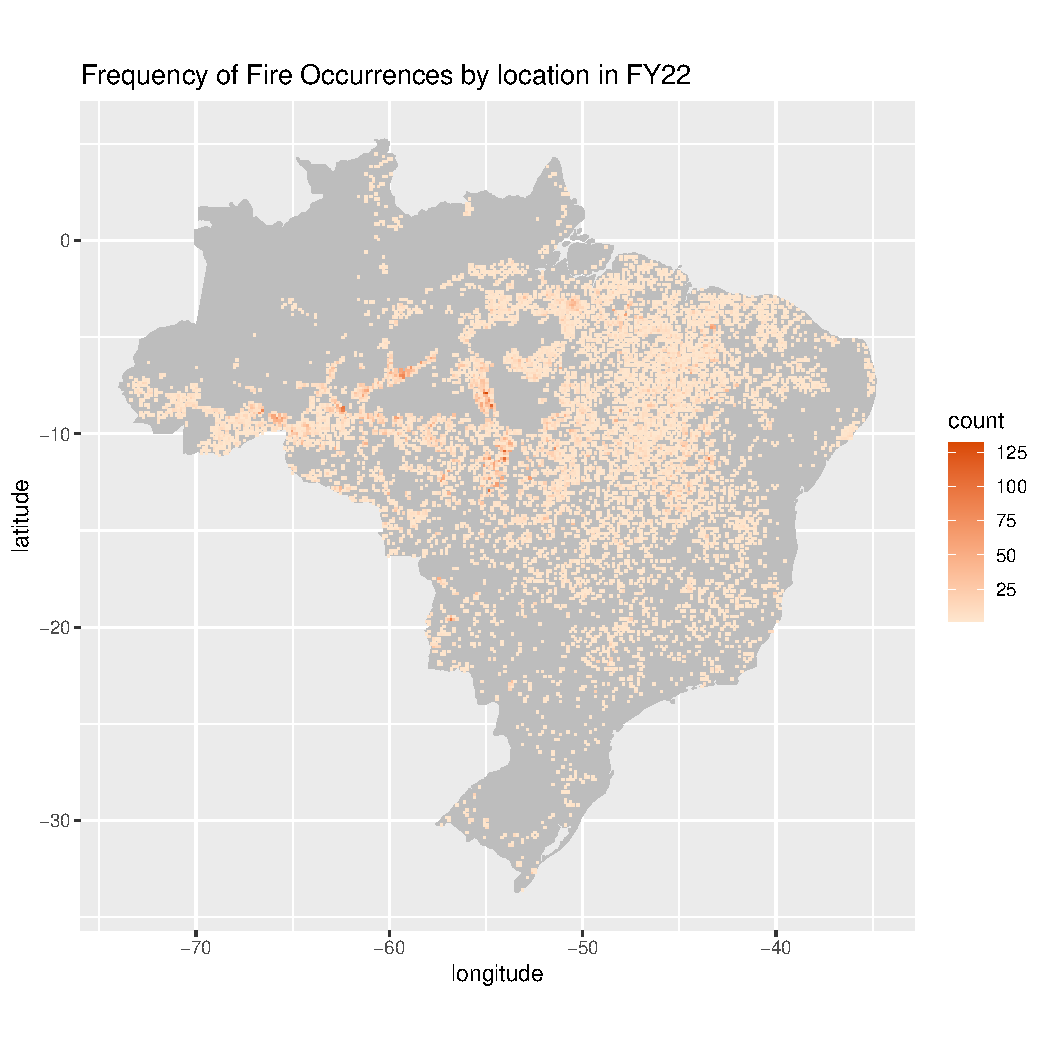
\includegraphics[width=\maxwidth]{figure/fire-by-location-fy22-1} 
\begin{kframe}\begin{alltt}
\hlcom{# Colour selection from: https://colorbrewer2.org/#type=sequential&scheme=Oranges&n=9}
\end{alltt}
\end{kframe}
\end{knitrout}



\begin{knitrout}
\definecolor{shadecolor}{rgb}{0.969, 0.969, 0.969}\color{fgcolor}\begin{kframe}
\begin{alltt}
\hlstd{heatmap_plot} \hlkwb{<-} \hlkwd{ggplot}\hlstd{(confident_fire_months_fy22,}
                       \hlkwd{aes}\hlstd{(}\hlkwc{x} \hlstd{= abb_month,} \hlkwc{y} \hlstd{=} \hlnum{2022}\hlstd{,} \hlkwc{fill} \hlstd{= count))} \hlopt{+}
  \hlkwd{geom_tile}\hlstd{(}\hlkwc{width} \hlstd{=} \hlnum{0.9}\hlstd{,} \hlkwc{height} \hlstd{=} \hlnum{1}\hlstd{)} \hlopt{+}  \hlcom{# Create the heatmap tiles}
  \hlkwd{scale_fill_gradient}\hlstd{(}\hlkwc{low} \hlstd{=} \hlstr{"white"}\hlstd{,} \hlkwc{high} \hlstd{=} \hlstr{"#d94801"}\hlstd{)} \hlopt{+}  \hlcom{# Customize the color scale}
  \hlkwd{labs}\hlstd{(}\hlkwc{title} \hlstd{=} \hlstr{"Frequency of Fire Occurrences by months in FY22"}\hlstd{,} \hlkwc{x} \hlstd{=} \hlstr{"Month"}\hlstd{,} \hlkwc{y} \hlstd{=} \hlstr{"FY22"}\hlstd{)} \hlopt{+}
  \hlkwd{theme}\hlstd{(}\hlkwc{panel.grid} \hlstd{=} \hlkwd{element_blank}\hlstd{() )}

\hlcom{# Display the heatmap}
\hlkwd{print}\hlstd{(heatmap_plot)}
\end{alltt}
\end{kframe}
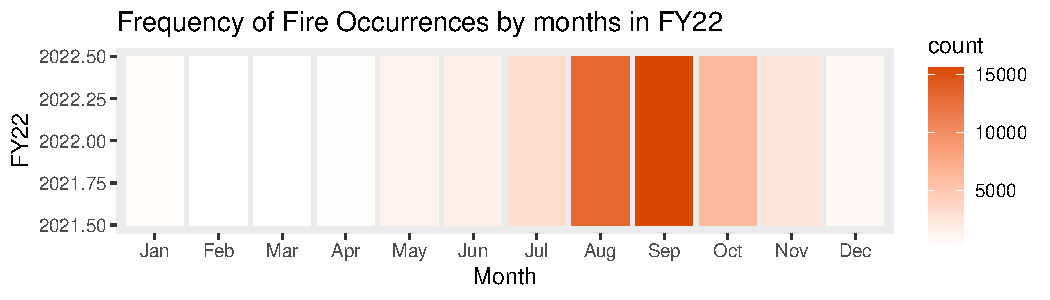
\includegraphics[width=\maxwidth]{figure/fire-by-months_fy22-1} 
\end{knitrout}
From the table, we can clearly see that August and September are the riskiest months in terms of fire hazard, whereas November to July hardly pose any risk at all. It's natural to ask the follow-up question: How does FY22 compare to previous years? Is it valid to claim that August and September are the fire hazard season?

\end{document}
